\documentclass[12pt]{report}
\usepackage[utf8]{inputenc}
\usepackage[russian]{babel}
%\usepackage[14pt]{extsizes}
\usepackage{listings}
\usepackage{graphicx}
\usepackage{amsmath,amsfonts,amssymb,amsthm,mathtools} 
\usepackage{pgfplots}
\usepackage{filecontents}
\usepackage{indentfirst}
\usepackage{eucal}
\usepackage{amsmath}
\usepackage{enumitem}
\frenchspacing

\usepackage{indentfirst} % Красная строка


%\usetikzlibrary{datavisualization}
%\usetikzlibrary{datavisualization.formats.functions}

\usepackage{amsmath}




% Для листинга кода:
\lstset{ %
language=haskell,                 % выбор языка для подсветки (здесь это С)
basicstyle=\small\sffamily, % размер и начертание шрифта для подсветки кода
numbers=left,               % где поставить нумерацию строк (слева\справа)
numberstyle=\tiny,           % размер шрифта для номеров строк
stepnumber=1,                   % размер шага между двумя номерами строк
numbersep=5pt,                % как далеко отстоят номера строк от подсвечиваемого кода
showspaces=false,            % показывать или нет пробелы специальными отступами
showstringspaces=false,      % показывать или нет пробелы в строках
showtabs=false,             % показывать или нет табуляцию в строках
frame=single,              % рисовать рамку вокруг кода
tabsize=2,                 % размер табуляции по умолчанию равен 2 пробелам
captionpos=t,              % позиция заголовка вверху [t] или внизу [b] 
breaklines=true,           % автоматически переносить строки (да\нет)
breakatwhitespace=false, % переносить строки только если есть пробел
escapeinside={\#*}{*)}   % если нужно добавить комментарии в коде
}

\usepackage[left=2cm,right=2cm, top=2cm,bottom=2cm,bindingoffset=0cm]{geometry}
% Для измененных титулов глав:
\usepackage{titlesec, blindtext, color} % подключаем нужные пакеты
\definecolor{gray75}{gray}{0.75} % определяем цвет
\newcommand{\hsp}{\hspace{20pt}} % длина линии в 20pt
% titleformat определяет стиль
\titleformat{\chapter}[hang]{\Huge\bfseries}{\thechapter\hsp\textcolor{gray75}{|}\hsp}{0pt}{\Huge\bfseries}


% plot
\usepackage{pgfplots}
\usepackage{filecontents}
\usetikzlibrary{datavisualization}
\usetikzlibrary{datavisualization.formats.functions}

\begin{document}
%\def\chaptername{} % убирает "Глава"
\thispagestyle{empty}
\begin{titlepage}
	\noindent \begin{minipage}{0.15\textwidth}
	
\includegraphics[width=\linewidth]{b_logo}
	\end{minipage}
	\noindent\begin{minipage}{0.9\textwidth}\centering
		\textbf{Министерство науки и высшего образования Российской Федерации}\\
		\textbf{Федеральное государственное бюджетное образовательное учреждение высшего образования}\\
		\textbf{~~~«Московский государственный технический университет имени Н.Э.~Баумана}\\
		\textbf{(национальный исследовательский университет)»}\\
		\textbf{(МГТУ им. Н.Э.~Баумана)}
	\end{minipage}
	
	\noindent\rule{18cm}{3pt}
	\newline\newline
	\noindent ФАКУЛЬТЕТ $\underline{\text{«Информатика и системы управления»}}$ \newline\newline
	\noindent КАФЕДРА $\underline{\text{«Программное обеспечение ЭВМ и информационные технологии»}}$\newline\newline\newline\newline\newline
	
	
	\begin{center}
		\noindent\begin{minipage}{1.3\textwidth}\centering
			\Large\textbf{  Отчёт по лабораторной работе №5}\newline
			\textbf{по дисциплине "Анализ алгоритмов"}\newline\newline
		\end{minipage}
	\end{center}
	
	\noindent\textbf{Тема} $\underline{\text{Конвейер}}$\newline\newline
	\noindent\textbf{Студент} $\underline{\text{Романов А.В.}}$\newline\newline
	\noindent\textbf{Группа} $\underline{\text{ИУ7-53Б}}$\newline\newline
	\noindent\textbf{Преподаватели} $\underline{\text{Волкова Л.Л., Строганов Ю.В.}}$\newline\newline\newline
	
	\begin{center}
		\vfill
		Москва~---~\the\year
		~г.
	\end{center}
\end{titlepage}


\tableofcontents

\newpage
\chapter*{Введение}
\addcontentsline{toc}{chapter}{Введение}

\section*{Задачи лабораторной работы}

В рамках выполнения работы необходимо решить следующие задачи:

\begin{itemize}
	\item 1
	\item 2
	\item 3
\end{itemize}

\chapter{Аналитическая часть}

\section{Описание задачи}


\section{Вывод}
	Вывод: аналит
\clearpage

\chapter{Конструкторская часть}

\section{Схемы алгоритмов}


\begin{figure}[h]
	\centering
	%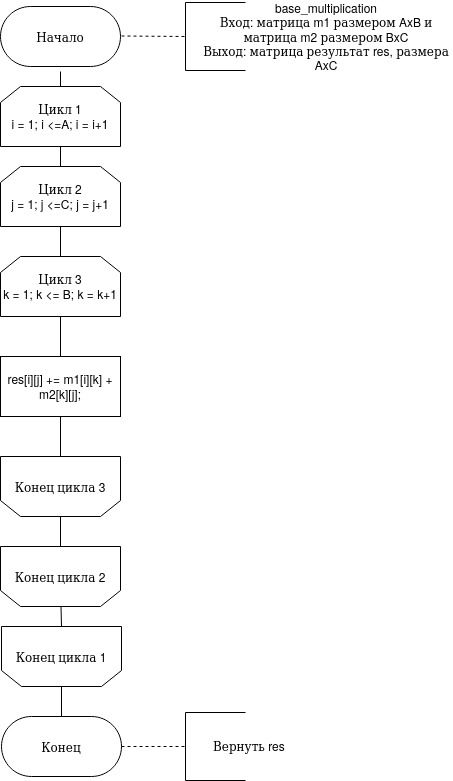
\includegraphics[scale=0.85]{base.jpg}
	\caption{Схема стандартного алгоритма умножения матриц.}
	\label{fig:mpr}
\end{figure}



\section{Вывод}
Вывод: конструктор

\chapter{Технологическая часть}

В данном разделе приведены средства реализации и листинги кода.

\section{Требование к ПО}

К программе предъявляется ряд требований:

\begin{itemize}
	\item 1
	\item 2
\end{itemize}

\section{Средства реализации}
Для реализации ПО я выбрал язык программирования Си \cite{C}. Данный выбор обусловлен высокой скоростью работы языка, а так же наличия инструментов для создания и эффективной работы с потоками.

\section{Реализация алгоритмов}


\begin{lstlisting}[label=some-code,caption=Функция умножения матриц обычным способом, language=C]
int main () {
	return 0;
}
\end{lstlisting}

\section{Тестовые данные}

\section{Вывод}

Вывод: тех

\chapter{Исследовательская часть}

\section{Технические характеристики}

Ниже приведены технические характеристики устройства, на котором было проведено тестирование ПО:

\begin{itemize}
	\item Операционная система: Debian \cite{debian} Linux \cite{linux} 11 <<bullseye>> 64-bit.
	\item Оперативная память: 12 GB.
	\item Процессор: Intel(R) Core(TM) i5-3550 CPU @ 3.30GHz
\cite{i5}.

\end{itemize}

\section{Время выполнения алгоритмов}


\begin{table} [h!]
	\caption{Таблица 123}
	\begin{center}
		\begin{tabular}{|c c c c|} 
		 	\hline
			Размер матрицы & Обычный & Параллельный 1 & Параллельный 2 \\  
		 	\hline
		 	64 & 11 569 478 & 4 423 500 & 4 399 005 \\
		 	\hline
		 	128 & 59 224 135 & 16 626 572 & 17 706 987 \\
		 	\hline
		 	256 & 354 152 337 & 98 670 198 & 96 640 191\\
		 	\hline
			512 & 2 719 059 760 & 755 595 299 & 751 307 775 \\
			\hline
			1024 & 26 717 252 997 & 7 347 757 065 & 7 489 450 509 \\
			\hline
		\end{tabular}
	\end{center}
\end{table}

\section{Вывод}

Вывод: исследовательская часть

\chapter*{Заключение}
\addcontentsline{toc}{chapter}{Заключение}

В рамках данной лабораторной работы:

\begin{itemize}
	\item 1
	\item 2
	\item 3
\end{itemize}

\addcontentsline{toc}{chapter}{Литература}

\bibliographystyle{utf8gost705u}  % стилевой файл для оформления по ГОСТу

\bibliography{51-biblio}          % имя библиографической базы (bib-файла)


\end{document}
